\documentclass[12pt,twocolumn]{article}
\usepackage{fullpage}
\usepackage[a4paper, margin=1.5cm, bottom=3cm]{geometry}
\usepackage[utf8]{inputenc}
\usepackage[T1]{fontenc}
\usepackage{hyperref}
\usepackage{url}
\usepackage[english,frenchb]{babel}
\usepackage{csquotes}
\usepackage{amsthm}
\newtheorem{prop}{Propriété}
\newtheorem{dfn}{Définition}
\usepackage{amssymb}
\usepackage{amsmath}
\usepackage{cancel}
\newcommand{\bigO}{\mathcal{O}}
\newcommand{\esN}{\mathbb{N}}
\newcommand{\esR}{\mathbb{R}}
\newcommand{\reg}{\mathcal{R}}
\newcommand{\es}{\emptyset}
\newcommand{\inc}{\subseteq}
\newcommand{\sm}{\setminus}
\usepackage{pgf,tikz}
\usetikzlibrary{arrows}
\usepackage[french,onelanguage]{algorithm2e}
\title{Projet de Structures de données II - Rapport final}
\author{Guillaume \textsc{Huysmans}}
\date{15 avril 2016}
\hypersetup{
	pdftitle={Projet de Structures de données II - Rapport final},
	pdfauthor={Guillaume \textsc{Huysmans}},
	pdfsubject={BSP, plan, binary space partition, Java, implementation},
	pdfkeywords={sdd2}}
\bibliographystyle{plain}
\begin{document}
\maketitle


\section{Arbre BSP}
Un arbre BSP (\textit{Binary Space Partition}) permet d'accéder efficacement
à des objets dans l'espace ou ici, le plan. Son principe est dérivé de celui
des arbres binaires. Chaque noeud interne représente une région $\reg$
du plan et est divisé en trois parties selon
une droite $D\equiv f(P)=aP_x+bP_y+c=0$ :
\begin{itemize}
	\item $d^-=\left\{f(P)<0 \; | \; P\in\reg\right\}$
	\item une liste de segments $s \inc D$
	\item $d^+=\left\{f(P)>0 \; | \; P\in\reg\right\}$
\end{itemize}

À une feuille de cet arbre, aucune droite ne sera associée et elle ne
contiendra qu'une liste de segments.


\section{Implémentation}
%fonctionnement des différentes structures et algorithmes utilisés
\subsection{Géométrie}
Les méthodes de projection et de calcul d'intersection ont été expérimentées dans
GeoGebra\footnote{\url{https://www.geogebra.org/?lang=fr}}
avant d'être implémentés en Java. Cela permettait de les tester de manière
interactive et de raisonner plus visuellement.

\begin{dfn}[Segment]\label{dfn:seg}
Soient $A,B\in\esR^2$.
Soient $x_m=\min(A_x,B_x), \; x_M=\max(A_x,B_x)$,
respectivement $y_m$ et $y_M$.
\begin{align*}
	[A,B]=\{(x,y)\in\esR^2 \; | \;
	& x_m\leq x\leq x_M \; \land \\
	& y_m\leq y\leq y_M \}
\end{align*}
\end{dfn}

\begin{prop}[Intersection segment--droite]\label{prop:inter}
Soient $A,B,A',B'\in\esR^2$.
\[
	[A,B] \cap A'B' = AB \cap A'B' \cap [A,B]
\]
\begin{proof}
\begin{align*}
	& AB \cap A'B' \cap [A,B] && \text{thèse} \\
	= & AB \cap [A,B] \cap A'B' && \text{commutativité} \\
	= & [A,B] \cap A'B' && [A,B] \inc AB
\end{align*}
\end{proof}
\end{prop}

\begin{figure}[h]
\center
\definecolor{uququq}{rgb}{0.25,0.25,0.25}
\definecolor{ttzzqq}{rgb}{0.2,0.6,0}
\definecolor{zzttqq}{rgb}{0.6,0.2,0}
\definecolor{qqqqff}{rgb}{0,0,1}
\begin{tikzpicture}[line cap=round,line join=round,>=triangle 45,x=1.0cm,y=1.0cm]
\clip(0.25,0.19) rectangle (4,6.4);
\fill[color=zzttqq,fill=zzttqq,fill opacity=0.1] (0.66,4.1) -- (2.3,4.1) -- (2.3,2.18) -- (0.66,2.18) -- cycle;
\fill[color=ttzzqq,fill=ttzzqq,fill opacity=0.1] (3.27,5.79) -- (1,5.79) -- (1,1) -- (3.27,1) -- cycle;
\draw (0.66,4.1)-- (2.3,2.18);
\draw [color=zzttqq] (0.66,4.1)-- (2.3,4.1);
\draw [color=zzttqq] (2.3,4.1)-- (2.3,2.18);
\draw [color=zzttqq] (2.3,2.18)-- (0.66,2.18);
\draw [color=zzttqq] (0.66,2.18)-- (0.66,4.1);
\draw (3.27,5.79)-- (1,1);
\draw [color=ttzzqq] (3.27,5.79)-- (1,5.79);
\draw [color=ttzzqq] (1,5.79)-- (1,1);
\draw [color=ttzzqq] (1,1)-- (3.27,1);
\draw [color=ttzzqq] (3.27,1)-- (3.27,5.79);
\begin{scriptsize}
\fill [color=qqqqff] (0.66,4.1) circle (1.5pt);
\draw[color=qqqqff] (0.81,4.34) node {$A$};
\fill [color=qqqqff] (2.3,2.18) circle (1.5pt);
\draw[color=qqqqff] (2.45,2.42) node {$B$};
\fill [color=qqqqff] (3.27,5.79) circle (1.5pt);
\draw[color=qqqqff] (3.44,6.03) node {$A'$};
\fill [color=qqqqff] (1,1) circle (1.5pt);
\draw[color=qqqqff] (0.94,0.83) node {$B'$};
\fill [color=uququq] (1.82,2.73) circle (1.5pt);
\draw[color=uququq] (2.01,2.86) node {$C$};
\end{scriptsize}
\end{tikzpicture}

\caption{Intersection de segments}
\end{figure}

Dans \texttt{core.Segment}, la méthode \texttt{contains}
implémente directement la définition \ref{dfn:seg}
et \texttt{contains} utilise la propriété \ref{prop:inter}.
L'intersection de droites se base sur la méthode de Cramer pour résoudre
un système de deux équations à deux inconnues.

La rotation de $P$ autour de $A$ d'un angle $\alpha$ est ainsi implémentée
dans \texttt{core.Point} :
\[
	(P-A) \times |P-A| \left(\begin{array}{cc}
	\cos\alpha & -\sin\alpha \\ \sin\alpha & \cos\alpha
	\end{array}\right)
	+ A
\]
On passe dans un repère centré sur $A$, on fait tourner $P$ autour de
la nouvelle origine puis on revient dans le repère d'où l'on est parti.

La hiérarchie des objets ne distingue pas un~point $P$ d'un vecteur $OP$.

\begin{prop}[Angle]
Le plus petit angle $\alpha$ entre les vecteurs $u$ et $v$ peut se calculer
à partir de leur produit scalaire :
\begin{align*}
	u.v = & |u|\times|v|\times\cos\alpha \\
	= & u_xv_x + u_yv_y
\end{align*}
De là, on isole aisément $\alpha$ :
\[
	\alpha = \cos^{-1}\left(\frac{u_xv_x + u_yv_y}{|u|\times|v|}\right)
\]
\end{prop}

La projection d'un point se fait en deux étapes : d'abord, on calcule l'angle
entre le vecteur le plus à gauche dans notre champ de vision ($t$) et celui
de la caméra au point visé ($d$). Ensuite, on refait le même calcul avec
le centre de notre champ de vision et $d$. En effet, un seul des deux résultats
ne suffit pas puisqu'on ne peut pas savoir de quel côté (positif ou négatif)
on se situe avec un simple $cos^{-1}$. On sait ainsi si le point est visible
(le rapport entre l'angle avec $u$ et le champ de vision est alors retourné)
ou trop loin d'un côté ou de l'autre ($\pm\infty$ est retourné).

\begin{figure}[h]
\center
\definecolor{ffqqqq}{rgb}{1,0,0}
\definecolor{qqcctt}{rgb}{0,0.8,0.2}
\definecolor{qqzzzz}{rgb}{0,0.6,0.6}
\definecolor{qqwuqq}{rgb}{0,0.39,0}
\definecolor{qqqqff}{rgb}{0,0,1}
\begin{tikzpicture}[line cap=round,line join=round,>=triangle 45,x=1.0cm,y=1.0cm]
\clip(1.25,1.13) rectangle (6.71,6.64);
\draw [shift={(1.52,3.08)},color=qqwuqq,fill=qqwuqq,fill opacity=0.1] (0,0) -- (-17.89:0.52) arc (-17.89:42.11:0.52) -- cycle;
\draw [->] (1.52,3.08) -- (6.46,4.14);
\draw [color=qqzzzz,domain=1.25:6.71] plot(\x,{(-24.65--4.94*\x)/-1.06});
\draw [->,color=qqcctt] (1.52,3.08) -- (4.7,1.37);
\draw [->,color=ffqqqq] (1.52,3.08) -- (5.27,6.47);
\draw [->,color=ffqqqq] (1.52,3.08) -- (6.33,1.53);
\begin{scriptsize}
\fill [color=qqqqff] (1.52,3.08) circle (1.5pt);
\draw[color=qqqqff] (1.58,2.94) node {$pov$};
\fill [color=qqqqff] (6.46,4.14) circle (1.5pt);
\draw[color=black] (3.92,3.86) node {$d$};
\fill [color=qqqqff] (4.7,1.37) circle (1.5pt);
\draw[color=qqqqff] (4.83,1.59) node {$p$};
\draw[color=qqwuqq] (1.72,2.72) node {$60\textrm{\degre}$};
\draw[color=qqcctt] (3.21,2.41) node {$u$};
\draw[color=ffqqqq] (3.38,4.95) node {$t$};
\draw[color=ffqqqq] (4,2.49) node {$b$};
\end{scriptsize}
\end{tikzpicture}

\caption{Projection d'un point}
\end{figure}

Un segment ne sera pas visible s'il est entièrement derrière la caméra,
c'est-à-dire du côté opposé au point qu'elle fixe. Sinon, il suffit de projeter
ses extrémités et de vérifier qu'elles ne sont pas au même endroit, ce qui
arrivera si la caméra est alignée avec un segment <<~sans épaisseur~>>.


\subsection{Architecture logicielle}
À la figure \ref{fig:core} sont représentées les relations importantes
entre les objets du noyau du logiciel. Un peintre est seulement chargé
de parcourir les segments dans le <<~bon ordre~>>. Il est utilisé pour
représenter la projection des segments mais également pour présenter la vue de
haut (où il y a moins de contraintes). Les heuristiques implémentent toutes une
même interface qui leur permet de donner l'indice du prochain segment à utiliser
et lors de l'initialisation de modifier la liste lue à partir de la scène.
Les \textit{free splits} n'étant qu'une amélioration de \texttt{Random}
(elle-même identique à l'initialisation près, comme dans \cite[p.~256]{cg}),
elle en hérite tout naturellement. Pour qu'elle fonctionne, le plus simple
pour moi était
d'ajouter à \texttt{Point} un indicateur disant qu'il s'agit d'une intersection.
Lorsque les deux extrémités d'un segment en sont, on peut l'utiliser sans
risquer que la droite qui le supporte n'en coupe un autre
\footnote{Nous faisons l'hypothèse comme dans \cite[p.~256]{cg}
que les segments ne se coupent pas}.
La projection est faite dans la classe abstraite du peintre puisque
cette opération nécessite des informations liées à la caméra
que nous ne calculerons qu'une fois.

\begin{figure}[h]
\center
\includegraphics[width=\columnwidth]{class.png}
\caption{Architecture du noyau}\label{fig:core}
\end{figure}

À la figure \ref{fig:ui} nous retrouvons le couplage entre les interfaces
utilisateur et le noyau du logiciel. \texttt{PainterCallback} permet au peintre
de nous rendre la main puisqu'on ne peut pas en Java 8 passer de fonctions en
paramètres.

\begin{figure}[h]
\center
\includegraphics[width=\columnwidth]{class-use.png}
\caption{Architecture de l'interface utilisateur}\label{fig:ui}
\end{figure}


\section{Mode d'emploi}
\subsection{TestUI}
Un nom de fichier peut être passé en paramètre afin de ne pas devoir le
sélectionner manuellement. Vous pouvez sélectionner une heuristique
(par défaut \texttt{First}) avant de lancer la construction de l'arbre BSP.
%FIXME pré-remplir le champ et ne pas utiliser First d'office !

Une fois l'arbre créé, deux représentations de la~scène sont présentées :
\begin{itemize}
\item à gauche, un arbre montrant les différents noeuds du BSP ainsi
	que le nombre de segments qu'ils contiennent;
\item à droite, une vue de haut.
	%Cette dernière est la première fois générée
	%n parcourant la liste des segments. Une fois que la caméra sera placée,
	%n <<~vrai peintre~>> travaille à partir du BSP.
\end{itemize}

Pour (dé)placer la caméra, il faut cliquer une première fois à la position sur
laquelle la placer et une seconde fois sur un point qu'elle fixe.

Pour déplacer la vue de haut, il faut modifier le code source (désolay). %FIXME

Une copie d'écran de TestUI est présentée à la figure \ref{fig:screen}.

\begin{figure}[h]
\center
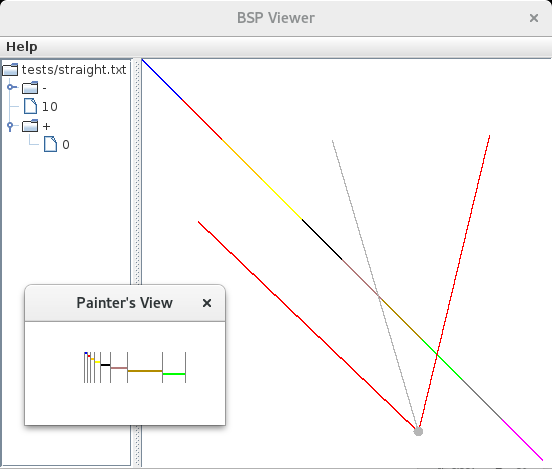
\includegraphics[width=\columnwidth]{ui.png} %FIXME
\caption{Copie d'écran de TestUI}\label{fig:screen}
\end{figure}


\subsection{TestCompare}
Comme pour l'interface fenêtrée,
un nom de fichier peut être passé en paramètre afin d'éviter la saisie
de la commande \texttt{load "scène.txt"} (notez la présence des guillemets).

Il est préférable d'utiliser \texttt{rlwrap -c}
\footnote{\texttt{rlwrap} est disponible dans les dépôts Debian.}
afin de profiter d'une autocomplétion des noms de fichiers et
des touches directionnelles autrement indisponibles puisque
l'entrée est seulement traitée ligne par ligne.

Les autres commandes disponibles sont :
\begin{itemize}
	\item \texttt{first} pour construire un BSP avec l'heuristique déterministe;
	\item \texttt{random} pour créer au hasard un arbre;
	\item \texttt{free} pour profiter des \textit{free splits};
	\item \texttt{test \underline{n}} pour créer $n$ BSP en utilisant chaque
		heuristique disponible;
	\item \texttt{exit}|\texttt{quit} pour quitter le programme.
\end{itemize}

L'utilisation type de TestCompare est présentée à la figure \ref{fig:cmp}.

\begin{figure}[h]
\begin{verbatim}
$ rlwrap -c \
  java -cp build ui.TestCompare \
  scenes/rectangles/rectanglesHuge.txt
>>> free
Algorithm         Time (ms)
BSP construction      12.74
Painter                0.38

Stats               Count
Height                 13
Nodes                 361
Segments            15609
\end{verbatim}
\caption{Utilisation type de TestCompare}\label{fig:cmp}
\end{figure}


\section{Résultats}
%donner et commenter les résultats de vos comparaison des heuristiques
Sur la figure \ref{fig:eL}, on observe que l'ordre des segments dans la
scène est bien meilleur que les autres examinés par \texttt{Random}. Cela vient
du fait que la scène est construite en commençant par l'extérieur...
La figure \ref{fig:eL-n} montre seulement la différence entre
les heuristiques non déterministes.
\begin{figure}[p]
\center
\includegraphics[width=\columnwidth]{../Rplots.pdf}%FIXME
\caption{\texttt{ellipsesLarge.txt}}\label{fig:eL}
\end{figure}
\begin{figure}[p]
\center
\includegraphics[width=\columnwidth]{../Rplots.pdf}%FIXME
\caption{\texttt{ellipsesLarge.txt} sans \texttt{First}}\label{fig:eL-n}
\end{figure}

Le fichier \texttt{rectanglesHuge.txt} n'a pas pu été traité tel quel puisqu'il
contenait des <<~segments~>> $[PQ]$ tels que $P=Q=(\pm250,0)$.


\section{Analyse de complexité}
\begin{algorithm}
\caption{peindre, décrit dans \cite[p.~255]{cg}}
\SetAlgoLined\DontPrintSemicolon
\KwData{$t, \; pov$}
\uIf{$t=\es$} {
	ne rien faire
}
\uElseIf{$(t^+=\es) \land (t^-=\es)$} {
	afficher chaque segment de $t_s$
}
\Else {
	$p$ = position de $pov$ par rapport à $t_D$ \;
	\uIf{$p>0$} {
		peindre $t^-$ depuis $pov$ \;
		afficher chaque segment de $t_s$ \;
		peindre $t^+$ depuis $pov$ \;
	}
	\uElseIf{$p<0$} {
		peindre $t^+$ depuis $pov$ \;
		afficher chaque segment de $t_s$ \;
		peindre $t^-$ depuis $pov$ \;
	}
	\Else {
		peindre $t^+$ depuis $pov$ \;
		peindre $t^-$ depuis $pov$ \;
	}
}
~
\end{algorithm}

Par feuille, il y a :
\begin{itemize}
	\item deux comparaisons en $\bigO(1)$
	\item l'affichage des segments qu'elle contient
\end{itemize}

Pour chaque noeud interne $t$, en ignorant les appels récursifs, on observe :
\begin{itemize}
	\item trois comparaisons en $\bigO(1)$
	\item un calcul en $\bigO(1)$
	\item dans le pire des cas :
		\begin{itemize}
			\item deux autres comparaisons en $\bigO(1)$
			\item l'affichage des segments dans $t_s$
		\end{itemize}
\end{itemize}

On observe que tous les noeuds seront visités une seule fois et que dans le pire
des cas, tous les segments seront peints. Il s'agit en fait d'un parcours
d'arbre, l'ordre n'a pas d'importance pour évaluer sa complexité. L'algorithme
s'exécute en $\bigO(n)$ avec $n$ le nombre de noeuds dans l'arbre
lorsque l'on ignore l'affichage des segments.

Il est prouvé dans \cite[p.~258]{cg} que
le nombre de fragments de segments obtenus après construction d'un BSP
est en $\bigO(s+2s\ln s)=\bigO(s\ln s)$ avec $s$, le nombre
de segments contenus dans la scène.

Globalement, dans le pire des cas, tous les noeuds sont parcourus et
tous les segments seront peints. Les complexités s'additionnent pour donner
$\bigO(n+s\ln s)$. Or lorsque $s\geq1$, on a toujours $n\leq s+2$ :
on travaille avec des autopartitions
tout en faisant attention aux cas extrêmes où il n'y a que deux segments.
On trouve ainsi $\bigO(s\ln s)$.
%FIXME imaginer pires cas (dessiner), tableau comme en cours ?


\section{Conclusion}
%apports, difficultés, comparaison théorie/pratique
Ce projet était pour moi l'occasion de découvrir une solution élégante à un
problème qui me semblait difficilement soluble en 3D avec beaucoup d'objets.
Il serait intéressant de généraliser les choses dans l'espace mais je doute
de disposer des connaissances nécessaires en géométrie pour y parvenir.
L'abréviation me disait quelque chose, c'est en fait aussi l'extension de
fichier des cartes dans Quake et ses dérivés puisque le moteur original utilise
(entre autres) cette structure de donnée afin de fonctionner efficacement
même sur des machines peu puissantes.

\texttt{StreamTokenizer} m'était jusque-là inconnu et il s'est avéré bien
pratique puisqu'il n'était ainsi plus nécessaire de découper en lexèmes
les commandes entrées par l'utilisateur.


\bibliography{compgeom}

\end{document}
